\documentclass{beamer}
\mode<presentation>{
  \usetheme{Boadilla}
  \usefonttheme[onlylarge]{structurebold}
  \usefonttheme[stillsansseriflarge]{serif}
  \setbeamerfont*{frametitle}{size=\normalsize,series=\bfseries}
  % \setbeamertemplate{navigation symbols}{}
  \setbeamercovered{transparent}
}
\usepackage[english]{babel}
\usepackage[latin1]{inputenc}
\usepackage{times}
\usepackage[T1]{fontenc}
\usepackage{amsmath}
\usepackage{amssymb}
\usepackage{esint}
\usepackage{hyperref}
\usepackage{tikz}
\usepackage{xkeyval}
\usepackage{xargs}
\usepackage{xcolor}
\usepackage{verbatim}
\usepackage{listings}
\usepackage{multimedia}
\usepackage{bm}
\usepackage{siunitx}
\usetikzlibrary{
  arrows,
  calc,
  decorations.pathmorphing,
  decorations.pathreplacing,
  decorations.markings,
  fadings,
  positioning,
  shapes,
  arrows.meta
}
\tikzset{
  mid arrow/.style={postaction={decorate,decoration={
        markings,
        mark=at position .5 with {\arrow[#1]{stealth}}
      }}},
  mid arrow2/.style={postaction={decorate,decoration={
        markings,
        mark=at position .5 with {\arrow[>=stealth]{><}}
      }}},
}

\usepgfmodule{oo}

\pgfdeclareradialshading{glow2}{\pgfpoint{0cm}{0cm}}{
  color(0mm)=(white);
  color(2mm)=(white);
  color(8mm)=(black);
  color(10mm)=(black)
}
\pgfdeclareradialshading{glow}{\pgfpoint{0cm}{0cm}}{
  color(0mm)=(white);
  color(5mm)=(white);
  color(9mm)=(black);
  color(10mm)=(black)
}

\begin{tikzfadingfrompicture}[name=glow fading]
  \shade [shading=glow] (0,0) circle (1);
\end{tikzfadingfrompicture}

\begin{tikzfadingfrompicture}[name=glow2 fading]
  \shade [shading=glow2] (0,0) circle (1);
\end{tikzfadingfrompicture}

\mode<handout>{
  \usepackage{pgfpages}
  \pgfpagesuselayout{4 on 1}[a4paper,landscape,border shrink=5mm]
  \setbeamercolor{background canvas}{bg=black!10}
}

\newcommand\pgfmathsinandcos[3]{%
  \pgfmathsetmacro#1{sin(#3)}%
  \pgfmathsetmacro#2{cos(#3)}%
}
\newcommand\LongitudePlane[3][current plane]{%
  \pgfmathsinandcos\sinEl\cosEl{#2} % elevation
  \pgfmathsinandcos\sint\cost{#3} % azimuth
  \tikzset{#1/.estyle={cm={\cost,\sint*\sinEl,0,\cosEl,(0,0)}}}
}
\newcommand\LatitudePlane[3][current plane]{%
  \pgfmathsinandcos\sinEl\cosEl{#2} % elevation
  \pgfmathsinandcos\sint\cost{#3} % latitude
  \pgfmathsetmacro\yshift{\cosEl*\sint}
  \tikzset{#1/.estyle={cm={\cost,0,0,\cost*\sinEl,(0,\yshift)}}} %
}
\newcommand\DrawLongitudeCircle[2][1]{
  \LongitudePlane{\angEl}{#2}
  \tikzset{current plane/.prefix style={scale=#1}}
  % angle of "visibility"
  \pgfmathsetmacro\angVis{atan(sin(#2)*cos(\angEl)/sin(\angEl))} %
  \draw[current plane] (\angVis:1) arc (\angVis:\angVis+180:1);
  \draw[current plane,dashed] (\angVis-180:1) arc (\angVis-180:\angVis:1);
}
\newcommand\DrawLatitudeCircleArrow[2][1]{
  \LatitudePlane{\angEl}{#2}
  \tikzset{current plane/.prefix style={scale=#1}}
  \pgfmathsetmacro\sinVis{sin(#2)/cos(#2)*sin(\angEl)/cos(\angEl)}
  % angle of "visibility"
  \pgfmathsetmacro\angVis{asin(min(1,max(\sinVis,-1)))}
  \draw[current plane,decoration={markings, mark=at position 0.6 with {\arrow{<}}},postaction={decorate},line width=.6mm] (\angVis:1) arc (\angVis:-\angVis-180:1);
  \draw[current plane,dashed,line width=.6mm] (180-\angVis:1) arc (180-\angVis:\angVis:1);
}
\newcommand\DrawLatitudeCircle[2][1]{
  \LatitudePlane{\angEl}{#2}
  \tikzset{current plane/.prefix style={scale=#1}}
  \pgfmathsetmacro\sinVis{sin(#2)/cos(#2)*sin(\angEl)/cos(\angEl)}
  % angle of "visibility"
  \pgfmathsetmacro\angVis{asin(min(1,max(\sinVis,-1)))}
  \draw[current plane] (\angVis:1) arc (\angVis:-\angVis-180:1);
  \draw[current plane,dashed] (180-\angVis:1) arc (180-\angVis:\angVis:1);
}
\newcommand\coil[1]{
  {\rh * cos(\t * pi r)}, {\apart * (2 * #1 + \t) + \rv * sin(\t * pi r)}
}
\makeatletter
\define@key{DrawFromCenter}{style}[{->}]{
  \tikzset{DrawFromCenterPlane/.style={#1}}
}
\define@key{DrawFromCenter}{r}[1]{
  \def\@R{#1}
}
\define@key{DrawFromCenter}{center}[(0, 0)]{
  \def\@Center{#1}
}
\define@key{DrawFromCenter}{theta}[0]{
  \def\@Theta{#1}
}
\define@key{DrawFromCenter}{phi}[0]{
  \def\@Phi{#1}
}
\presetkeys{DrawFromCenter}{style, r, center, theta, phi}{}
\newcommand*\DrawFromCenter[1][]{
  \setkeys{DrawFromCenter}{#1}{
    \pgfmathsinandcos\sint\cost{\@Theta}
    \pgfmathsinandcos\sinp\cosp{\@Phi}
    \pgfmathsinandcos\sinA\cosA{\angEl}
    \pgfmathsetmacro\DX{\@R*\cost*\cosp}
    \pgfmathsetmacro\DY{\@R*(\cost*\sinp*\sinA+\sint*\cosA)}
    \draw[DrawFromCenterPlane] \@Center -- ++(\DX, \DY);
  }
}
\newcommand*\DrawFromCenterText[2][]{
  \setkeys{DrawFromCenter}{#1}{
    \pgfmathsinandcos\sint\cost{\@Theta}
    \pgfmathsinandcos\sinp\cosp{\@Phi}
    \pgfmathsinandcos\sinA\cosA{\angEl}
    \pgfmathsetmacro\DX{\@R*\cost*\cosp}
    \pgfmathsetmacro\DY{\@R*(\cost*\sinp*\sinA+\sint*\cosA)}
    \draw[DrawFromCenterPlane] \@Center -- ++(\DX, \DY) node {#2};
  }
}
\makeatother

\newcommand\drawlens[3]{
  % 1: center (x, y)
  % 2: size
  % 3: angle
  \begin{scope}[shift={#1}]
    \node[rotate={#3}] at (0, 0) {\scalebox{#2}{\includegraphics[width=2cm]{fadings/lens.png}}};
  \end{scope}
}
\newcommand\drawwaveplate[3]{
  % 1: center (x, y)
  % 2: size
  % 3: angle
  \begin{scope}[shift={#1}]
    \node[rotate={#3}] at (0, 0)
    {\scalebox{#2}{\includegraphics[width=2cm]{fadings/waveplate.png}}};
  \end{scope}
}
\newcommand\drawaom[4]{
  % 1: center (x, y)
  % 2: xsize
  % 3: ysize
  % 4: angle
  \begin{scope}[shift={#1}]
    \node[rotate={#4}] at (0, 0)
    {\scalebox{#2}[#3]{\includegraphics[width=2cm,height=2cm]{fadings/aom.png}}};
  \end{scope}
  \begin{scope}[rotate around={#4:#1}]
    \fill[orange, even odd rule, opacity=0.8]
    ($#1 + ({#2}, 0)$) arc (0:360:{#2} and {#3})
    -- ($#1 + ({#2}, {#3})$) -- ($#1 + (-{#2}, {#3})$) -- ($#1 + (-{#2}, -{#3})$)
    -- ($#1 + ({#2}, -{#3})$) --cycle;
    \draw ($#1 + ({#2}, {#3})$) -- ($#1 + (-{#2}, {#3})$) -- ($#1 + (-{#2}, -{#3})$)
    -- ($#1 + ({#2}, -{#3})$) --cycle;
  \end{scope}
}
\newcommand\drawpbs[3]{
  % 1: center (x, y)
  % 2: size
  % 3: angle
  \begin{scope}
    \begin{scope}
      \clip[rotate around={#3:#1}] ($#1 - ({#2}, {#2})$) rectangle ($#1 + ({#2}, {#2})$);
      \begin{scope}[transform canvas={shift={#1}, rotate=#3}]
        \node[rotate=-90] at (0, 0)
        {\scalebox{#2}{\includegraphics[width=2cm,
            height=2cm]{fadings/pbs.png}}};
        \draw[line width=1] (-{#2}, -{#2}) -- ({#2}, {#2});
      \end{scope}
    \end{scope}
    % Make sure the frame is not clipped
    \draw[rotate around={#3:#1}] ($#1 - ({#2}, {#2})$) rectangle ($#1 + ({#2}, {#2})$);
  \end{scope}
}
\newcommand\drawnonpbs[3]{
  % 1: center (x, y)
  % 2: size
  % 3: angle
  \begin{scope}
    \begin{scope}
      \clip[rotate around={#3:#1}] ($#1 - ({#2}, {#2})$) rectangle ($#1 + ({#2}, {#2})$);
      \begin{scope}[transform canvas={shift={#1}, rotate=#3}]
        \node[rotate=-90] at (0, 0)
        {\scalebox{#2}{\includegraphics[width=2cm,
            height=2cm]{fadings/non_pbs.png}}};
        \draw[line width=1] (-{#2}, -{#2}) -- ({#2}, {#2});
      \end{scope}
    \end{scope}
    % Make sure the frame is not clipped
    \draw[rotate around={#3:#1}] ($#1 - ({#2}, {#2})$) rectangle ($#1 + ({#2}, {#2})$);
  \end{scope}
}

% not mandatory, but I though it was better to set it blank
\setbeamertemplate{headline}{}
\def\beamer@entrycode{\vspace{-\headheight}}

\tikzstyle{snakearrow} = [decorate, decoration={pre length=0.2cm,
  post length=0.2cm, snake, amplitude=.4mm,
  segment length=2mm},thick, ->]

%% document-wide tikz options and styles

\tikzset{%
  % >=latex, % option for nice arrows
  inner sep=0pt,%
  outer sep=2pt,%
  mark coordinate/.style={inner sep=0pt,outer sep=0pt,minimum size=3pt,
    fill=black,circle}%
}
\tikzset{
  % Define standard arrow tip
  >=stealth',
  % Define style for boxes
  punkt/.style={
    rectangle,
    rounded corners,
    draw=black, very thick,
    text width=8em,
    minimum height=2.5em,
    text centered},
}

\tikzset{onslide/.code args={<#1>#2}{%
    \only<#1>{\pgfkeysalso{#2}}
    % \pgfkeysalso doesn't change the path
  }}
\tikzset{alt/.code args={<#1>#2#3}{%
    \alt<#1>{\pgfkeysalso{#2}}{\pgfkeysalso{#3}}
    % \pgfkeysalso doesn't change the path
  }}
\tikzset{temporal/.code args={<#1>#2#3#4}{%
    \temporal<#1>{\pgfkeysalso{#2}}{\pgfkeysalso{#3}}{\pgfkeysalso{#4}}
    % \pgfkeysalso doesn't change the path
  }}

\makeatletter
\newbox\@backgroundblock
\newenvironment{backgroundblock}[2]{%
  \global\setbox\@backgroundblock=\vbox\bgroup%
  \unvbox\@backgroundblock%
  \vbox to0pt\bgroup\vskip#2\hbox to0pt\bgroup\hskip#1\relax%
}{\egroup\egroup\egroup}
\addtobeamertemplate{background}{\box\@backgroundblock}{}
\makeatother

% \def\timeleft{15:00->14:55}

\title{Optics}
\date{Oct. 18, 2022}
\author{Yichao Yu}
\institute{Journal Club}

\ifpdf
  % Ensure reproducible output
  \pdfinfoomitdate=1
  \pdfsuppressptexinfo=-1
  \pdftrailerid{}
  \hypersetup{
    pdfcreator={},
    pdfproducer={}
  }
\fi

\begin{document}

{
  \begin{frame}{}
    \titlepage
  \end{frame}
}

\begin{frame}{Geometrical optics}
  \begin{center}
    \visible<1->{
      \textbf{Useful for $>90\%$ of calculation.}\\
    }
    \visible<2->{
      \begin{columns}
        \column{7cm}
        \begin{block}{Exceptions}
          \begin{itemize}
          \item Focus
          \item<3-> Long propagation
          \item<4-> Diffraction optical elements\\
            e.g. gratings.
          \end{itemize}
        \end{block}
      \end{columns}
    }
  \end{center}
\end{frame}

\begin{frame}{Ideal Lens}
  \begin{center}
    \begin{tikzpicture}
      \visible<-7>{
        \draw[red, line width=1.5] (-2.25, 0.8) -- (4.5, -1.6);
        \draw[red, line width=1.5] (-2.25, 0.8) -- (0, -1.6) -- (4.5, -1.6);
        \draw[red, line width=1.5] (-2.25, 0.8) -- (0, 0.8) -- (4.5, -1.6);

        \draw[dashed, line width=2] (-5, 0) -- (5, 0);
        \draw[<->,>=stealth, line width=1.5] (0, 2) -- (0, -2);
        \fill (-1.5, 0) circle (0.1) node[below=0.16] {F};
        \fill (1.5, 0) circle (0.1) node[below=0.16] {F};
        \draw[->, line width=1] (-2.25, 0) -- (-2.25, 0.8);
        \draw[->, line width=2] (4.5, 0) -- (4.5, -1.6);

        \node[below=0.05] at (-0.6, 0) {$f$};
        \node[below=0.02] at (0.8, 0) {$f$};
      }
      \visible<8->{
        \draw[red, line width=1.5] (-3.05, 0.8) -- (-0.8, 0);
        \draw[red, line width=1.5] (0.2, 0) -- (4.7, -1.6);
        \draw[red, line width=1.5] (-3.05, 0.8) -- (-0.8, -1.6);
        \draw[red, line width=1.5] (0.2, -1.6) -- (4.7, -1.6);
        \draw[red, line width=1.5] (-3.05, 0.8) -- (-0.8, 0.8);
        \draw[red, line width=1.5] (0.2, 0.8) -- (4.7, -1.6);

        \draw[dashed, line width=2] (-5, 0) -- (5, 0);
        \draw[dashed, line width=1.5] (-0.8, -2) -- (-0.8, 2) node[above] {$H_1$};
        \draw[dashed, line width=1.5] (0.2, -2) -- (0.2, 2) node[above] {$H_2$};
        \fill (-2.3, 0) circle (0.1) node[below=0.16] {F};
        \fill (1.7, 0) circle (0.1) node[below=0.16] {F};
        \draw[->, line width=1] (-3.05, 0) -- (-3.05, 0.8);
        \draw[->, line width=2] (4.7, 0) -- (4.7, -1.6);

        \node[below=0.05] at (-1.4, 0) {$f$};
        \node[below=0.02] at (1.0, 0) {$f$};
      }

      \visible<2-3>{
        \draw[green!70!black,decoration={brace,amplitude=10pt},decorate,line width=1]
        (-2.2, 0.9) -- node[above=0.32] {$u$} (-0.05, 0.9);
        \draw[green!70!black,decoration={brace,amplitude=10pt},decorate,line width=1]
        (0.05, 0.9) -- node[above=0.32] {$v$} (4.45, 0.9);
        \draw[dashed, line width=1.5, opacity=0.3] (4.5, 0.8) -- (4.5, 0);
      }

      \visible<4-5>{
        \draw[blue!70!black,decoration={brace,mirror,amplitude=5pt},
        decorate,line width=1]
        (-2.25, -0.6) -- node[below=0.2] {$x_1$} (-1.5, -0.6);
        \draw[blue!70!black,decoration={brace,amplitude=10pt},
        decorate,line width=1]
        (1.5, 0.2) -- node[above=0.32] {$x_2$} (4.5, 0.2);
      }
      \visible<2-3>{
        \node[green!70!black] at (0, -2.7) {$\dfrac{1}{u}+\dfrac{1}{v}=\dfrac{1}{f}$};
        \visible<3>{
          \node[green!70!black] at (0, -3.7) {$M=\dfrac{v}{u}$};
        }
      }
      \visible<4-5>{
        \node[blue!70!black] at (0, -2.7) {$x_1x_2=f^2$};
        \visible<5>{
          \node[blue!70!black] at (0, -3.7) {$M=\dfrac{f}{x_1}=\dfrac{x_2}{f}=\sqrt{\dfrac{x_2}{x_1}}$};
        }
      }
      \visible<6-7>{
        \node[below,align=center,text width=6cm] at (0, -2.3) {
          \begin{tabular}{rl}
            Conjugate plane:\!\!&\!\!Perfect image under ray optics\\
            \visible<7->{Principal planes:}\!\!&\!\!\visible<7->{Conjugate plane where $M=1$}
          \end{tabular}
        };
      }
    \end{tikzpicture}
  \end{center}
\end{frame}

\begin{frame}{Spherical lens}
  \begin{center}
    \begin{tikzpicture}
      \draw[dashed, line width=2] (-5, 0) -- (5, 0);
      \visible<-3>{
        \draw[line width=0.8,fill=cyan!60!blue,fill opacity=0.3]
        (0, -2) arc (-11.536959032815489:11.536959032815489:10)
        arc ({180-23.578178478201835}:{180+23.578178478201835}:5);
      }
      \visible<4>{
        \draw[line width=0.8,fill=cyan!60!blue,fill opacity=0.3]
        (0, -2) -- (0, 2)
        arc ({180-23.578178478201835}:{180+23.578178478201835}:5);
      }

      \visible<1>{
        \draw[line width=0.8,dashed]
        (0, 2) arc (11.536959032815489:18:10);
        \path[line width=0.8,dashed]
        (0, 2) arc (11.536959032815489:16:10) coordinate (R1);
        \draw[<-,>=stealth,line width=1.2] (R1) -- node[sloped, above] {$R_1$} ++(18:-1);

        \draw[line width=0.8,dashed]
        (0, 2) arc (180-23.578178478201835:180-30.5:10);
        \path[line width=0.8,dashed]
        (0, 2) arc (180-23.578178478201835:180-28:10) coordinate (R2);
        \draw[<-,>=stealth,line width=1.2] (R2) -- node[sloped, above] {$R_2$} ++(-28:1);
      }

      \visible<2-4>{
        \draw[red, line width=1.5] (-5, 0.3) -- (0, 0.3) -- (5, -0.2);
        \draw[red, line width=1.5] (-5, -0.3) -- (0, -0.3) -- (5, 0.2);
      }
      \visible<3>{
        \draw[red!20!orange, line width=1] (-5, 0.6) -- (0, 0.6) -- (2.7, 0) -- (4.5, -0.4);
        \draw[red!20!orange, line width=1] (-5, -0.6) -- (0, -0.6) -- (2.7, 0) -- (4.5, 0.4);

        \draw[red!20!orange, line width=1] (-5, 0.9) -- (0, 0.9) -- (2.4, 0) -- (4.0, -0.6);
        \draw[red!20!orange, line width=1] (-5, -0.9) -- (0, -0.9) -- (2.4, 0) -- (4.0, 0.6);

        \draw[red!20!orange, line width=1] (-5, 1.2) -- (0, 1.2) -- (2.1, 0) -- (3.5, -0.8);
        \draw[red!20!orange, line width=1] (-5, -1.2) -- (0, -1.2) -- (2.1, 0) -- (3.5, 0.8);
      }
      \visible<2-4>{
        \fill (3, 0) circle (0.08) node[below=0.16] {F};
      }
    \end{tikzpicture}
  \end{center}
\end{frame}

\begin{frame}{Aspherical lens}
  \begin{center}
    \begin{columns}
      \column{3cm}
      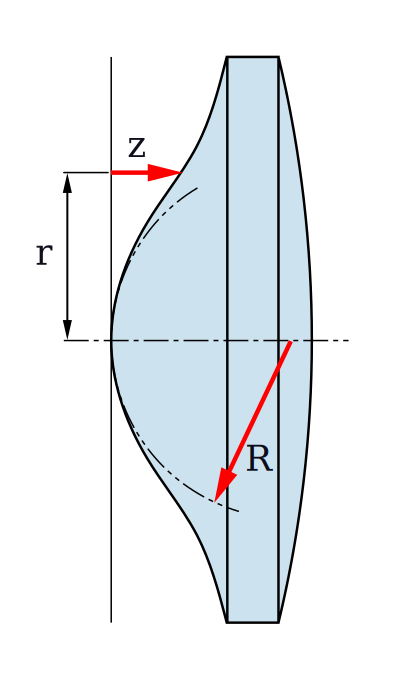
\includegraphics[width=2.5cm]{imgs/Asphere.pdf}
      \column{6cm}
      \visible<2->{
        \begin{block}{Use cases}
          \begin{itemize}
          \item Collimation
          \item Fiber coupling
          \end{itemize}
        \end{block}
      }
    \end{columns}
  \end{center}
\end{frame}

\begin{frame}{Other lens types}
  \begin{center}
    \begin{columns}
      \column{5.2cm}
      \visible<1->{
        \begin{block}{Reflective}
          \begin{itemize}
          \item No chromatic shift
          \item Can be aspherical
          \item More difficult beam path layout
          \end{itemize}
        \end{block}
      }
      \column{5.2cm}
      \visible<2->{
        \begin{block}{Lens set}
          \begin{itemize}
          \item Could fix chromatic shift
          \item Could fix monochromatic aberration
          \item Better surface quality
          \item May not be UV compatible
          \end{itemize}
        \end{block}
      }
    \end{columns}
  \end{center}
\end{frame}

\begin{frame}{Fiber coupling}
  \begin{center}
    \begin{tikzpicture}
      \visible<-3>{
        \node at (0, 0) {\textbf{Collimation}};

        \draw[dashed,line width=0.8,opacity=0.2] (-4, -2) -- (4, -2);

        \visible<2->{
          \draw[blue, dashed, line width=0.5] (-1, -1) -- (1, -2) -- (-1, -3);
          \draw[blue, line width=0.5] (0.2, -2) arc (180:180-26.56505117707799:0.8)
          node[midway,left] {$\theta$};
          \draw[blue,->,>=stealth,line width=0.5] (-2.5, -1.5) -- (-2.5, -1);
          \node[blue] at (-2.5, -2) {$d$};
          \draw[blue,->,>=stealth,line width=0.5] (-2.5, -2.5) -- (-2.5, -3);
        }

        \draw[line width=1] (4, -2.2) -- (1, -2.2) -- (1, -1.8) -- (4, -1.8);
        \draw[red, line width=0.7, domain=-2:0,smooth,variable=\x]
        (-4, -1) -- plot ({\x + 1}, {-2 + sqrt(0.2^2 + (\x / 2)^2)});
        \draw[red, line width=0.7, domain=-2:0,smooth,variable=\x]
        (-4, -3) -- plot ({\x + 1}, {-2 - sqrt(0.2^2 + (\x / 2)^2)});
        \draw[<->,>=stealth, line width=1.5] (-1, -3.3) -- (-1, -0.7);

        \visible<3->{
          \node[blue,below] at (0, -4) {$d\approx 2f\tan\theta$};
        }
      }
      \visible<4->{
        \node at (0, 0) {\textbf{Alignment}};

        \visible<5>{
          \node at (-2.8, -3) {
\includegraphics[width=4.2cm]{imgs/opt_sym.pdf}};
        }
        \visible<6>{
          \node at (-2.8, -3) {\includegraphics[width=4.2cm]{imgs/opt_sym_point.pdf}};
        }
        \visible<7->{
          \node at (-2.8, -3) {\includegraphics[width=4.2cm]{imgs/opt_sym_align.pdf}};
        }
        \visible<8>{
          \node at (2.8, -3) {\includegraphics[width=4.2cm]{imgs/opt_asym.pdf}};
        }
        \visible<9>{
          \node at (2.8, -3) {\includegraphics[width=4.2cm]{imgs/opt_asym_axis.pdf}};
        }
        \visible<10>{
          \node at (2.8, -3) {\includegraphics[width=4.2cm]{imgs/opt_asym_point.pdf}};
        }
        \visible<11>{
          \node at (2.8, -3) {\includegraphics[width=4.2cm]{imgs/opt_asym_naive.pdf}};
        }
        \visible<12->{
          \node at (2.8, -3) {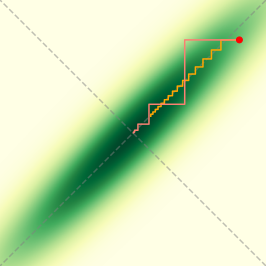
\includegraphics[width=4.2cm]{imgs/opt_asym_jump.pdf}};
        }
      }
    \end{tikzpicture}
  \end{center}
\end{frame}

\begin{frame}[t]{Polarization\visible<2->{: Polarizers}}
  \begin{center}
    \begin{columns}[t]
      \begin{column}{3.9cm}
        \visible<3->{
          \centering
          \textbf{PBS Cubes}\\
          \visible<4->{
            \begin{itemize}
            \item Based on coating
            \item Easy to use for both polarizations
            \item OK loss (few \%)
            \item low-mid extinction
            \item Wavelength dependent
            \end{itemize}
          }
        }
      \end{column}
      \begin{column}{3.9cm}
        \visible<5->{
          \centering
          \textbf{Prisms}\\
          \visible<6->{
            \begin{itemize}
            \item Based on birefringence
            \item Non 90 reflection angle
            \item Low loss
            \item High extinction
            \item Etaloning
            \item Broadband
            \end{itemize}
          }
        }
      \end{column}
      \begin{column}{3.9cm}
        \visible<7->{
          \centering
          \textbf{Thin film}\\
          \visible<8->{
            \begin{itemize}
            \item Based on absorption
            \item Easy to use\\
              (minimal change to beam)
            \item High loss
            \item High extinction
            \item Broadband
            \end{itemize}
          }
        }
      \end{column}
    \end{columns}
  \end{center}
\end{frame}

\begin{frame}[t]{Polarization: Waveplates}
  \begin{center}
    \begin{tikzpicture}
      \node at (0, 0) {$\Delta\phi=\dfrac{2\pi nl}{\lambda}$};
      \visible<2>{
        \node at (-2.5, -1.5) {Half WP: $\Delta\phi=\dfrac{\pi}{2}$};
        \node at (2.5, -1.5) {Quarter WP: $\Delta\phi=\dfrac{\pi}{4}$};
      }
      \visible<3->{
        \node at (-2.5, -1.5) {Half WP: $\Delta\phi=2n\pi+\dfrac{\pi}{2}$};
        \node at (2.5, -1.5) {Quarter WP: $\Delta\phi=2n\pi+\dfrac{\pi}{4}$};
      }
      \visible<4->{
        \node at (0, -3) {Zero-th order WP: $n=0$};
      }
      \visible<5->{
        \node at (0, -4.5) {Other WP type: Achromatic, ``Magic''};
      }
    \end{tikzpicture}
  \end{center}
\end{frame}

\begin{frame}{Polarization: Effect of reflection}
  \begin{center}
    \begin{columns}[t]
      \column{5.5cm}
      \begin{block}{Normal incident}
        \begin{itemize}
        \item $\pi$ phase shift
        \item No effect on relative amplitude
        \end{itemize}
      \end{block}
      \vspace{0.2cm}
      \visible<2->{
        \begin{center}
          \begin{tikzpicture}
            \draw[red, line width=1] (-2, 2) -- (0, 0) -- (2, 2);

            \fill[red] (-0.8, 0.8) circle (0.1);
            \fill[red] (-1.5, 1.5) circle (0.1);
            \draw[<->,>=stealth,red,line width=0.8]
            (-0.8 - 0.4, 0.8 - 0.4) -- (-0.8 + 0.4, 0.8 + 0.4);
            \draw[<->,>=stealth,red,line width=0.8]
            (-1.5 - 0.4, 1.5 - 0.4) -- (-1.5 + 0.4, 1.5 + 0.4);

            \fill[red] (0.8, 0.8) circle (0.1);
            \fill[red] (1.5, 1.5) circle (0.1);
            \draw[<->,>=stealth,red,line width=0.8]
            (0.8 + 0.4, 0.8 - 0.4) -- (0.8 - 0.4, 0.8 + 0.4);
            \draw[<->,>=stealth,red,line width=0.8]
            (1.5 + 0.4, 1.5 - 0.4) -- (1.5 - 0.4, 1.5 + 0.4);

            \draw[<->,>=stealth,red,line width=0.8]
            (-1.7, -1 - 0.4) --
            node[right=0.36] {$p$-polarization}
            (-1.7, -1 + 0.4);
            \fill[<->,>=stealth,red,line width=0.8]
            (-1.7, -2) circle (0.1)
            node[right=0.36] {$s$-polarization};

            \draw[line width=2] (-2.5, 0) -- (2.5, 0);
          \end{tikzpicture}
        \end{center}
      }
      \vspace{1cm}
      \column{5.5cm}
      \visible<3->{
        \begin{block}{Simple surface}
          \begin{itemize}
          \item (metal or dielectric)
          \item $\pi$ phase shift
          \item Change relative amplitude
          \end{itemize}
        \end{block}
      }
      \vspace{0.3cm}
      \visible<4->{
        \begin{block}{Coating}
          \begin{itemize}
          \item ``Arbitrary'' phase shift
          \item Change relative amplitude
          \item (dielectric mirror, dichroics)
          \end{itemize}
        \end{block}
      }
    \end{columns}
  \end{center}
\end{frame}

\begin{frame}[t]{Electro-optic modulator (EOM)\visible<2->{ \footnotesize i.e. electrically variable waveplate}}
  \begin{center}
    \begin{tikzpicture}
      \visible<3,10->{
        \node at (0, 0) {$n=n_0+\alpha E$};
      }
      \visible<4-9>{
        \node at (0, 0) {$n_{i}={n_0}_{i}+\alpha_i^j E_j$};
      }
      \visible<5-7>{
        \node[align=center,text width=8cm,below] at (0, -0.1) {
          \begin{block}{DC EOM: adjustable waveplate}
            \begin{itemize}
            \item<6-> Rotate polarization
            \item<6-> (with polarizer) Turn beam on/off
            \item<7-> Temperature drift compensation
            \end{itemize}
          \end{block}
        };
      }
      \visible<8->{
        \node[align=center,text width=8cm,below] at (0, -0.1) {
          \begin{block}{AC EOM: phase/polarization modulation}
            \begin{itemize}
            \item<9-> Polarization modulation
            \item<9-> Power modulation
            \item<10-> Phase modulation/sideband
            \item<12-> Asymmetric sideband\visible<14->{: sawtooth drive}
            \end{itemize}
          \end{block}
        };
      }
      \visible<11>{
        \node[align=center,text width=8cm,below] at (0, -3) {
          \begin{align*}
            \phi=&\phi_0+\beta\sin(\omega t)\\
            \tilde{A}=&A_0\exp(\mathrm{i}\phi)\\
            =&\tilde{A_0}\exp(\mathrm{i}\beta\sin(\omega t))\\
            =&\tilde{A_0}\sum_{n=-\infty}^{\infty}J_{n}(\beta)\exp(\mathrm{i}n\omega t)
          \end{align*}
        };
      }
      \visible<13>{
        \node[align=center,below] at (0, -4) {
          $\phi=\phi_0+\omega t$
        };
      }
      \visible<14->{
        \node[align=center,below] at (0, -4) {
          $\phi=mod(\phi_0+\omega t, 2\pi)$
        };
      }
    \end{tikzpicture}
  \end{center}
\end{frame}

\begin{frame}[t]{Acousto-optic modulator (AOM)\visible<2->{ \footnotesize i.e. dynamic/moving grating}}
  \begin{center}
    \begin{tikzpicture}
      \visible<3-5>{
        \draw[red,line width=15] (-4, 0) -- (4, 0);
        \draw[red,line width=15] (0, 0) -- (4, 2);
        \draw[red,line width=15] (0, 0) -- (4, 1);
        \draw[red,line width=15] (0, 0) -- (4, -1);
        \draw[red,line width=15] (0, 0) -- (4, -2);

        \draw[line width=1] (0, 1.5) -- (0, 1.4);
        \draw[line width=1] (0, 1.3) -- (0, 1.2);
        \draw[line width=1] (0, 1.1) -- (0, 1.0);
        \draw[line width=1] (0, 0.9) -- (0, 0.8);
        \draw[line width=1] (0, 0.7) -- (0, 0.6);
        \draw[line width=1] (0, 0.5) -- (0, 0.4);
        \draw[line width=1] (0, 0.3) -- (0, 0.2);
        \draw[line width=1] (0, 0.1) -- (0, 0);
        \draw[line width=1] (0, -0.1) -- (0, -0.2);
        \draw[line width=1] (0, -0.3) -- (0, -0.4);
        \draw[line width=1] (0, -0.5) -- (0, -0.6);
        \draw[line width=1] (0, -0.7) -- (0, -0.8);
        \draw[line width=1] (0, -0.9) -- (0, -1.0);
        \draw[line width=1] (0, -1.1) -- (0, -1.2);
        \draw[line width=1] (0, -1.3) -- (0, -1.4);
        \draw[line width=1] (0, -1.5) -- (0, -1.6);

        \draw[line width=0.8] (0, 0.95) -- (-1, 0.95);
        \draw[line width=0.8] (0, 1.15) -- (-1, 1.15);
        \draw[->,line width=1,>=stealth] (-0.5, 1.55) -- node[left=0.1] {$d$} (-0.5, 1.15);
        \draw[->,line width=1,>=stealth] (-0.5, 0.55) -- (-0.5, 0.95);

        \draw[dashed,line width=1] (-5, 0) -- (5, 0);
        \draw[dashed,line width=1] (0, 0) -- (5, 1.25);
        \draw[line width=1] (1.6, 0) arc (0:14.036243467926479:1.6)
        node[midway,right] {$\theta$};

        \node at (0, -2.5) {$d\sin\theta_n=n\lambda$};

        \visible<4>{
          \node[above] at (0, 1.5) {$T(x)$};
          \node[below,align=center,text width=8cm] at (0, -2.5) {
            \begin{align*}
              T(x)=&\sum_na_n\exp\left(\mathrm{i}\frac{2n\pi x}{d}\right)
            \end{align*}
          };
        }

        \visible<5->{
          \node[above] at (0, 1.5) {$T(x- d \omega t/2\pi)$};
          \node[below,align=center,text width=8cm] at (0, -2.5) {
            \begin{align*}
              T(x)=&\sum_na_n\exp\left(\mathrm{i}\frac{2n\pi (x- d \omega t/2\pi)}{d}\right)\\
              =&\sum_na_n\exp\left(\mathrm{i}\frac{2n\pi x}{d}-\mathrm{i}n\omega t\right)
            \end{align*}
          };
        }
      }
      \visible<6->{
        \draw[red,line width=15] (-4, 0) -- (4, 0);
        \draw[red,line width=15] (0, 0) -- (4, -1);
        \foreach \i in {-5, ..., 5} {
          \draw[line width=1] (-1 + \i * 0.15 * 0.12310562561766054, 0.12310562561766054 + \i * 0.15) --
          ++(2, -2 * 0.12310562561766054);
        }
        \draw[dashed,line width=1] (-5, 0) -- (5, 0);
        \draw[dashed,line width=1] (0, 0) -- (5, -1.25);
      }
    \end{tikzpicture}
  \end{center}
\end{frame}

\begin{frame}[t]{Acousto-optic modulator (AOM) \footnotesize i.e. dynamic/moving grating}
  \begin{center}
    \begin{tikzpicture}
      \node at (2.75, -1.5) {\textbf{Double Pass}};
      % PBS input
      \draw[red,line width=1.6,mid arrow] (0, -2) -- (0, -3.5 + 0.5);
      \draw[red,line width=1.6] (0, -3.5 + 0.5) -- (0, -3.5);
      % AOM input
      \draw[red,line width=1.6] (0, -3.5) -- (0.6, -3.5);
      \draw[red,line width=1.6,mid arrow2] (0.6, -3.5) -- (2, -3.5);
      % DP
      \draw[red,line width=1.6,mid arrow2] (2, -3.5) -- (4.5, -4.1);
      \draw[red,line width=1.6] (4.5, -4.1) -- (4.95, -4.1);
      \draw[red,line width=1.6,mid arrow2] (4.95, -4.1) -- (7, -4.1);
      % output
      \draw[red,line width=1.6] (0, -3.5) -- (-0.95, -3.5);
      \draw[red,line width=1.6,mid arrow] (-0.95, -3.5) -- (-1.5, -3.5);

      % PBS
      \drawpbs{(0, -3.5)}{0.7}{90}
      \node[blue!40!cyan,below,align=center] at (0, -3.5 - 0.7) {\large PBS};
      % AOM
      \drawaom{(2, -3.5)}{1}{0.5}{90}
      \node[rotate=90,align=center] at (2, -3.5) {\large AOM};
      % QWP
      \drawwaveplate{(3.9, -3.5)}{1}{90}
      \node[blue!80!black,above] at (3.9, -3.5 + 0.8) {\large $\lambda/4$};
      % lens
      \drawlens{(4.5, -3.5)}{1}{90}
      % mirror
      \draw[line width=3] (7, -3.5 - 0.2) -- (7, -3.5 - 0.9);

      \visible<2->{
        \node at (2.75, -5.5) {\textbf{Tandem}};

        % AOM 1 input
        \draw[red,line width=1.6,mid arrow] (-2.5, -7) -- (-1.15, -7);
        \draw[red,line width=1.6] (-1.15, -7) -- (-1, -7);
        % AOM 1 output
        \draw[red,line width=1.6,mid arrow] (-1, -7) -- (2.75, -7 - 0.7);
        % AOM 2 input
        \draw[red,line width=1.6,mid arrow] (2.75, -7 - 0.7) -- (6.5, -7);
        % AOM 1 output
        \draw[red,line width=1.6] (6.5, -7) -- (7.2, -7);
        \draw[red,line width=1.6,mid arrow] (7.2, -7) -- (8, -7);

        % AOM 1
        \drawaom{(-1, -7)}{1}{0.5}{90}
        \node[rotate=90,align=center] at (-1, -7) {\large AOM 1};
        % lens
        \drawlens{(2.75, -7)}{1}{90}
        % AOM 2
        \drawaom{(6.5, -7)}{1}{0.5}{90}
        \node[rotate=90,align=center] at (6.5, -7) {\large AOM 2};
      }
    \end{tikzpicture}
  \end{center}
\end{frame}

\begin{frame}{AOM vs EOM}
  \begin{center}
    \begin{tikzpicture}
      \fill[opacity=0] (-5.8, -3.7) rectangle (5.8, 3.7);

      \draw[line width=1] (0, -3.7) -- (0, 3.7);
      \node[below] at (-2.9, 3.7) {\bf AOM};
      \node[below] at (2.9, 3.7) {\bf EOM};

      \visible<2->{
        \node[below] at (-2.9, 3.1) {$40-2000\mathrm{MHz}$};
        \node[below] at (2.9, 3.1) {$\mathrm{DC}-40\mathrm{GHz}$};
      }

      \visible<3->{
        \node[below] at (-2.9, 2.5) {Tunable (AOBD vs AOM)};
        \node[below] at (2.9, 2.5) {Tunable (if not resonant)};
      }

      \visible<4->{
        \node[below, align=center, text width=5.8cm]
        at (-2.9, 1.9) {Good suppression of wrong order};
        \node[below, align=center, text width=5.8cm]
        at (2.9, 1.9) {Bad suppression of wrong order};
      }

      \visible<5->{
        \node[below, align=center, text width=5.8cm]
        at (-2.9, 1.3) {No/little polarization modulation};
        \node[below, align=center, text width=5.8cm]
        at (2.9, 1.3) {Support polarization modulation};
      }

      \visible<6->{
        \node[below, align=center, text width=5.8cm]
        at (-2.9, 0.7) {Multiple frequencies in single beam\\
        (Requires multiple AOMs)};
        \node[below, align=center, text width=5.8cm]
        at (2.9, 0.7) {Multiple frequencies in single beam};
      }

      \visible<7->{
        \node[below, align=center, text width=5.8cm]
        at (-2.9, -0.4) {Steer beam with frequency};
        \node[below, align=center, text width=5.8cm]
        at (2.9, -0.4) {Cannot steer beam};
      }

      \visible<8->{
        \node[below, align=center, text width=5.8cm]
        at (-2.9, -1.0) {Switching implies frequency shift\\
        (Can shift back with another AOM)};
        \node[below, align=center, text width=5.8cm]
        at (2.9, -1.0) {Switching without frequency shift (DC)};
      }

      \visible<9->{
        \node[below, align=center, text width=5.8cm]
        at (-2.9, -2.1) {Slow ($\mu s$)};
        \node[below, align=center, text width=5.8cm]
        at (2.9, -2.1) {Fast ($ns$)};
      }
    \end{tikzpicture}
  \end{center}
\end{frame}

\end{document}
